% move all configuration stuff into one file so we can focus on the content
\documentclass[aspectratio=169,hyperref={pdfpagelabels=false,colorlinks=true,linkcolor=white,urlcolor=lightblue},xcolor={table},t]{beamer}

%%%%%%%%%%%%%%%%%%%%%%%%%%%%%%%%%%%%%%%%%%%%%%%%%%%%%%%%%%%%%%%%%%%%%%%%%%%%%%%%%%
%%%%%%%%%%%%%%%%%%%%%%%%%%%%%%%%%%%%%%%%%%%%%%%%%%%%%%%%%%%%%%%%%%%%%%%%%%%%%%%%%%
% packages
\usepackage{pict2e}
\usepackage{epic}
\usepackage{amsmath,amsfonts,amssymb}
\usepackage{units}
\usepackage{fancybox}
\usepackage[absolute,overlay]{textpos} 
%\usepackage[table]{xcolor}
\usepackage{animate}
\usepackage{gensymb}
%\usepackage{graphicx}
%\usepackage{longtable}
\usepackage{multirow}
\usepackage{silence}
\usepackage{tikz}
\usepackage[backend=bibtex,style=ieee]{biblatex}
\AtEveryCitekey{\iffootnote{\tiny}{}}
%\addbibresource{include/references}



% fontsize
\let\Tiny=\tiny

%%%%%%%%%%%%%%%%%%%%%%%%%%%%%%%%%%%%%%%%%%%%%%%%%%%%%%%%%%%%%%%%%%%%%%%%%%%%%%%%%%
%%%%%%%%%%%%%%%%%%%%%%%%%%%%%%%%%%%%%%%%%%%%%%%%%%%%%%%%%%%%%%%%%%%%%%%%%%%%%%%%%%
% warnings
\pdfsuppresswarningpagegroup=1
\WarningFilter{biblatex}{Patching footnotes failed}
\WarningFilter{latexfont}{Font shape}
\WarningFilter{latexfont}{Some font shapes}
\WarningFilter{gensymb}{Not defining}


%%%%%%%%%%%%%%%%%%%%%%%%%%%%%%%%%%%%%%%%%%%%%%%%%%%%%%%%%%%%%%%%%%%%%%%%%%%%%%%%%%
%%%%%%%%%%%%%%%%%%%%%%%%%%%%%%%%%%%%%%%%%%%%%%%%%%%%%%%%%%%%%%%%%%%%%%%%%%%%%%%%%%
% colors
\definecolor{gtgold}{rgb}{.914, .664, 0} %0e7eed {rgb}{0.88,0.66,1,0.06} [234, 170, 0]/256 %96caff
\definecolor{darkgray}{rgb}{.15, .15, .15}
\definecolor{lightblue}{HTML}{0e7eed}
\definecolor{highlight}{rgb}{0, 0, 1} %_less!40

%%%%%%%%%%%%%%%%%%%%%%%%%%%%%%%%%%%%%%%%%%%%%%%%%%%%%%%%%%%%%%%%%%%%%%%%%%%%%%%%%%
%%%%%%%%%%%%%%%%%%%%%%%%%%%%%%%%%%%%%%%%%%%%%%%%%%%%%%%%%%%%%%%%%%%%%%%%%%%%%%%%%%
% relative paths
\graphicspath{{../graph/}}


%%%%%%%%%%%%%%%%%%%%%%%%%%%%%%%%%%%%%%%%%%%%%%%%%%%%%%%%%%%%%%%%%%%%%%%%%%%%%%%%%%
%%%%%%%%%%%%%%%%%%%%%%%%%%%%%%%%%%%%%%%%%%%%%%%%%%%%%%%%%%%%%%%%%%%%%%%%%%%%%%%%%%
% units
\setlength{\unitlength}{1mm}

%%%%%%%%%%%%%%%%%%%%%%%%%%%%%%%%%%%%%%%%%%%%%%%%%%%%%%%%%%%%%%%%%%%%%%%%%%%%%%%%%%
%%%%%%%%%%%%%%%%%%%%%%%%%%%%%%%%%%%%%%%%%%%%%%%%%%%%%%%%%%%%%%%%%%%%%%%%%%%%%%%%%%
% math
\DeclareMathOperator*{\argmax}{argmax}
\DeclareMathOperator*{\argmin}{argmin}
\DeclareMathOperator*{\atan}{atan}
\DeclareMathOperator*{\arcsinh}{arcsinh}
\DeclareMathOperator*{\sign}{sign}
\DeclareMathOperator*{\tcdf}{tcdf}
\DeclareMathOperator*{\si}{sinc}
\DeclareMathOperator*{\princarg}{princarg}
\DeclareMathOperator*{\arccosh}{arccosh}
\DeclareMathOperator*{\hwr}{HWR}
\DeclareMathOperator*{\flip}{flip}
\DeclareMathOperator*{\sinc}{sinc}
\DeclareMathOperator*{\floor}{floor}
\newcommand{\e}{{e}}
\newcommand{\jom}{\mathrm{j}\omega}
\newcommand{\jOm}{\mathrm{j}\Omega}
\newcommand   {\mat}[1]    		{\boldsymbol{\uppercase{#1}}}		%bold
\renewcommand {\vec}[1]    		{\boldsymbol{\lowercase{#1}}}		%bold

%%%%%%%%%%%%%%%%%%%%%%%%%%%%%%%%%%%%%%%%%%%%%%%%%%%%%%%%%%%%%%%%%%%%%%%%%%%%%%%%%%
%%%%%%%%%%%%%%%%%%%%%%%%%%%%%%%%%%%%%%%%%%%%%%%%%%%%%%%%%%%%%%%%%%%%%%%%%%%%%%%%%%
% media9
\newcommand{\includeaudio}[1]{
\href{run:audio/#1.mp3}{
\includegraphics[width=5mm, height=5mm]{graph/SpeakerIcon}}}

\newcommand{\includeanimation}[4]{{\begin{center}
                        \animategraphics[autoplay,loop,scale=.7]{#4}{animation/#1-}{#2}{#3}        
                        \end{center}
                        \addreference{matlab source: \href{https://github.com/alexanderlerch/ACA-Plots/blob/master/matlab/animate#1.m}{matlab/animate#1.m}}}
                        \inserticon{video}}
                        
%%%%%%%%%%%%%%%%%%%%%%%%%%%%%%%%%%%%%%%%%%%%%%%%%%%%%%%%%%%%%%%%%%%%%%%%%%%%%%%%%%
%%%%%%%%%%%%%%%%%%%%%%%%%%%%%%%%%%%%%%%%%%%%%%%%%%%%%%%%%%%%%%%%%%%%%%%%%%%%%%%%%%
% other commands
\newcommand{\question}[1]{%\vspace{-4mm}
                          \setbeamercovered{invisible}
                          \begin{columns}[T]
                            \column{.9\textwidth}
                                \textbf{#1}
                            \column{.1\textwidth}
                                \vspace{-8mm}
                                \begin{flushright}
                                     
\includegraphics[width=.9\columnwidth]{graph/question_mark}
                                \end{flushright}
                                \vspace{6mm}
                          \end{columns}\pause\vspace{-12mm}}

\newcommand{\toremember}[1]{
                        \inserticon{lightbulb}
                        }

\newcommand{\matlabexercise}[1]{%\vspace{-4mm}
                          \setbeamercovered{invisible}
                          \begin{columns}[T]
                            \column{.8\textwidth}
                                \textbf{matlab exercise}: #1
                            \column{.2\textwidth}
                                \begin{flushright}
                                     \includegraphics[scale=.5]{graph/logo_matlab}
                                \end{flushright}
                                %\vspace{6mm}
                          \end{columns}}

\newcommand{\addreference}[1]{  
                  
                    \begin{textblock*}{\baselineskip }(.98\paperwidth,.5\textheight) %(1.15\textwidth,.4\textheight)
                         \begin{minipage}[b][.5\paperheight][b]{1cm}%
                            \vfill%
                             \rotatebox{90}{\tiny {#1}}
                        \end{minipage}
                   \end{textblock*}
                    }
                    
\newcommand{\figwithmatlab}[1]{
                    \begin{figure}
                        \centering
                        \includegraphics[scale=.7]{#1}
                        %\label{fig:#1}
                    \end{figure}
                    
                    \addreference{matlab source: \href{https://github.com/alexanderlerch/MUSI-6202/blob/main/matlab/plot#1.m}{plot#1.m}}}
\newcommand{\figwithref}[2]{
                    \begin{figure}
                        \centering
                        \includegraphics[scale=.7]{#1}
                        \label{fig:#1}
                    \end{figure}
                    
                    \addreference{#2}}  
                                    
\newcommand{\inserticon}[1]{
                    \begin{textblock*}{100mm}(14.5cm,7.5cm)
                        \includegraphics[height=.8cm,keepaspectratio]{graph/#1}
                    \end{textblock*}}            

%%%%%%%%%%%%%%%%%%%%%%%%%%%%%%%%%%%%%%%%%%%%%%%%%%%%%%%%%%%%%%%%%%%%%%%%%%%%%%%%%%
%%%%%%%%%%%%%%%%%%%%%%%%%%%%%%%%%%%%%%%%%%%%%%%%%%%%%%%%%%%%%%%%%%%%%%%%%%%%%%%%%%
% counters
\newcounter{i}
\newcounter{j}
\newcounter{iXOffset}
\newcounter{iYOffset}
\newcounter{iXBlockSize}
\newcounter{iYBlockSize}
\newcounter{iYBlockSizeDiv2}
\newcounter{iXBlockSizeDiv2}
\newcounter{iDistance}

\newcommand{\IEEELink}{https://ieeexplore.ieee.org/servlet/opac?bknumber=9965970}



\subtitle{Part 19: Modulated Effects}

%%%%%%%%%%%%%%%%%%%%%%%%%%%%%%%%%%%%%%%%%%%%%%%%%%%%%%%%%%%%%%%%%%%%%%%%%%%%
\begin{document}
    % generate title page
	\title[]{Digital Signal Processing for Music}   
\author[alexander lerch]{alexander lerch} 
%\institute{~}
%\date[Alexander Lerch]{}
\titlegraphic{\vspace{-16mm}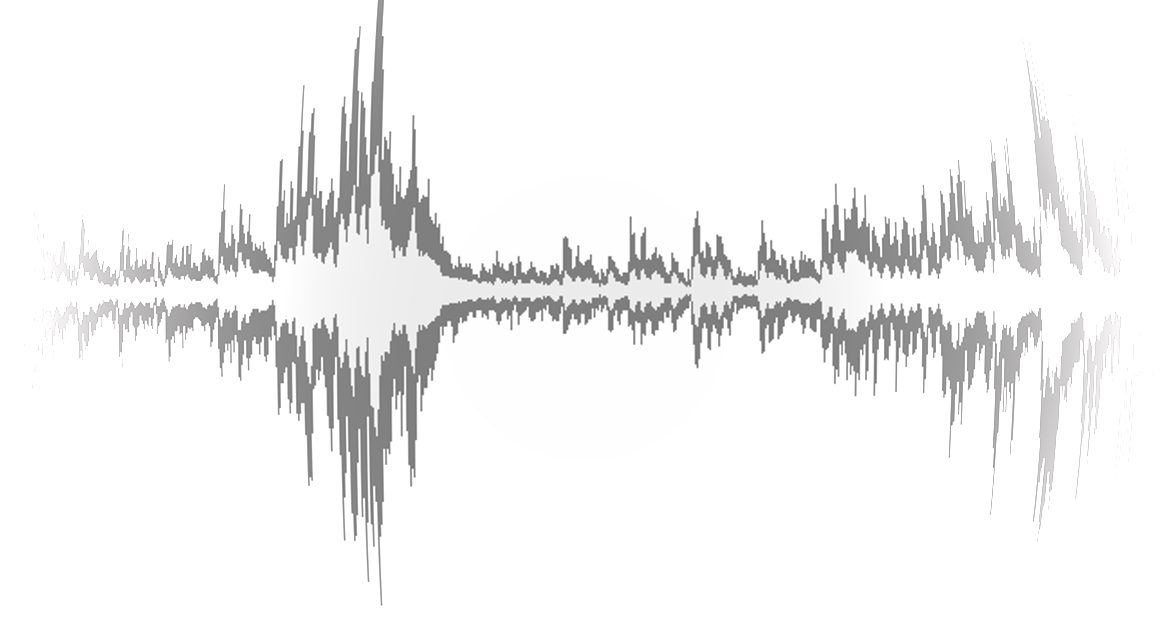
\includegraphics[width=\textwidth,height=3cm]{title}}


\begin{frame}
    \titlepage
    %\vspace{-5mm}
    \begin{flushright}
        \href{http://www.gtcmt.gatech.edu}{
\includegraphics[height=.8cm,keepaspectratio]{../shared/Logo_GTCMT_black}}
    \end{flushright}
\end{frame}


    \section[intro]{introduction}
        \begin{frame}{modulated effects}{introduction}
			
			\begin{itemize}
                \item   modulated effects belong to the probably oldest class of audio effects
                \item   often used for guitars
				\item<2->	\textbf{examples}
					\begin{itemize}
						\item	delay-line modulation:
                            \begin{itemize}
                                \item Vibrato
                                \item   Chorus, Flanger
                            \end{itemize}
                        \item   other
                            \begin{itemize}
                                \item Phaser
                                \item   Wah-Wah
                            \end{itemize}
					\end{itemize}
			\end{itemize}
		\end{frame}

    \section{delay line}
		\begin{frame}{modulated effects}{introduction: delay line}
			\begin{figure}
				\begin{center}
				\begin{picture}(30,10)

					%boxes
					\put(10,0){\framebox(10,10){\footnotesize{$z^{-M}$}}}

					%lines horizontal
					\put(0,5){\vector(1,0){10}}
					\put(20,5){\vector(1,0){10}}

					%text
					\put(0,8){\footnotesize{\shortstack[c]{x(i)}}}
					\put(30,8){\footnotesize{\shortstack[c]{y(i)}}}

				\end{picture}
				\end{center}
			\end{figure}
			
			\pause
			\textbf{implementation}
			\begin{figure}
				\begin{center}
				\begin{picture}(120,50)
					%boxes
					\setcounter{iXBlockSize}{15}
					\setcounter{iYBlockSize}{6}
					\setcounter{iYOffset}{40}
					\setcounter{iXOffset}{0}
					
					
					\put(10,50){\footnotesize{\shortstack[c]{input (write)}}}
					\put(85,50){\footnotesize{\shortstack[c]{output (read)}}}
					\put(0,\value{iYOffset}){\footnotesize{\shortstack[c]{i}}}
					\addtocounter{iXOffset}{10}
					\put(\value{iXOffset}, \value{iYOffset}){\framebox(\value{iXBlockSize},\value{iYBlockSize}){\tiny{$x_{i-1}$}}}
					\addtocounter{iXOffset}{\value{iXBlockSize}}
					\put(\value{iXOffset}, \value{iYOffset}){\framebox(\value{iXBlockSize},\value{iYBlockSize}){\tiny{$x_{i-2}$}}}
					\addtocounter{iXOffset}{\value{iXBlockSize}}
					\put(\value{iXOffset}, \value{iYOffset}){\framebox(\value{iXBlockSize},\value{iYBlockSize}){\tiny{$x_{i-3}$}}}
					\addtocounter{iXOffset}{\value{iXBlockSize}}
					\put(\value{iXOffset}, \value{iYOffset}){\framebox(\value{iXBlockSize},\value{iYBlockSize}){\tiny{$\ldots$}}}
					\addtocounter{iXOffset}{\value{iXBlockSize}}
					\put(\value{iXOffset}, \value{iYOffset}){\framebox(\value{iXBlockSize},\value{iYBlockSize}){\tiny{$x_{i-M+1}$}}}
					\addtocounter{iXOffset}{\value{iXBlockSize}}
					\put(\value{iXOffset}, \value{iYOffset}){\framebox(\value{iXBlockSize},\value{iYBlockSize}){\tiny{$x_{i-M}$}}}
					\addtocounter{iXOffset}{\value{iXBlockSize}}
		  
					\pause
					\put(20, 39){\vector(1,-1){7}}
					\put(80, 39){\vector(1,-1){7}}
					\put(35, 39){\vector(1,-1){7}}

					\addtocounter{iYOffset}{-\value{iXBlockSize}}
					\setcounter{iXOffset}{0}
					\put(0,\value{iYOffset}){\footnotesize{\shortstack[c]{i+1}}}
					\addtocounter{iXOffset}{10}
					\put(\value{iXOffset}, \value{iYOffset}){\framebox(\value{iXBlockSize},\value{iYBlockSize}){\tiny{$x_{i}$}}}
					\addtocounter{iXOffset}{\value{iXBlockSize}}
					\put(\value{iXOffset}, \value{iYOffset}){\framebox(\value{iXBlockSize},\value{iYBlockSize}){\tiny{$x_{i-1}$}}}
					\addtocounter{iXOffset}{\value{iXBlockSize}}
					\put(\value{iXOffset}, \value{iYOffset}){\framebox(\value{iXBlockSize},\value{iYBlockSize}){\tiny{$x_{i-2}$}}}
					\addtocounter{iXOffset}{\value{iXBlockSize}}
					\put(\value{iXOffset}, \value{iYOffset}){\framebox(\value{iXBlockSize},\value{iYBlockSize}){\tiny{$\ldots$}}}
					\addtocounter{iXOffset}{\value{iXBlockSize}}
					\put(\value{iXOffset}, \value{iYOffset}){\framebox(\value{iXBlockSize},\value{iYBlockSize}){\tiny{$x_{i-M+2}$}}}
					\addtocounter{iXOffset}{\value{iXBlockSize}}
					\put(\value{iXOffset}, \value{iYOffset}){\framebox(\value{iXBlockSize},\value{iYBlockSize}){\tiny{$x_{i-M+1}$}}}
					\addtocounter{iXOffset}{\value{iXBlockSize}}
		   
					\pause
					\put(20, 24){\vector(1,-1){7}}
					\put(80, 24){\vector(1,-1){7}}
					\put(35, 24){\vector(1,-1){7}}
		 
					\addtocounter{iYOffset}{-\value{iXBlockSize}}
					\setcounter{iXOffset}{0}
					\put(0,\value{iYOffset}){\footnotesize{\shortstack[c]{i+2}}}
					\addtocounter{iXOffset}{10}
					\put(\value{iXOffset}, \value{iYOffset}){\framebox(\value{iXBlockSize},\value{iYBlockSize}){\tiny{$x_{i+1}$}}}
					\addtocounter{iXOffset}{\value{iXBlockSize}}
					\put(\value{iXOffset}, \value{iYOffset}){\framebox(\value{iXBlockSize},\value{iYBlockSize}){\tiny{$x_{i}$}}}
					\addtocounter{iXOffset}{\value{iXBlockSize}}
					\put(\value{iXOffset}, \value{iYOffset}){\framebox(\value{iXBlockSize},\value{iYBlockSize}){\tiny{$x_{i-1}$}}}
					\addtocounter{iXOffset}{\value{iXBlockSize}}
					\put(\value{iXOffset}, \value{iYOffset}){\framebox(\value{iXBlockSize},\value{iYBlockSize}){\tiny{$\ldots$}}}
					\addtocounter{iXOffset}{\value{iXBlockSize}}
					\put(\value{iXOffset}, \value{iYOffset}){\framebox(\value{iXBlockSize},\value{iYBlockSize}){\tiny{$x_{i-M+3}$}}}
					\addtocounter{iXOffset}{\value{iXBlockSize}}
					\put(\value{iXOffset}, \value{iYOffset}){\framebox(\value{iXBlockSize},\value{iYBlockSize}){\tiny{$x_{i-M+2}$}}}
					\addtocounter{iXOffset}{\value{iXBlockSize}}
					
				\end{picture}
				\end{center}
			\end{figure}
		\end{frame}

		\begin{frame}{modulated effects}{introduction: ring buffer}
            \vspace{-7mm}\begin{columns}
            \column{.75\linewidth}
			\begin{itemize}
				\item	\textbf{idea}
					\begin{itemize}
						\item	do not move buffer contents
						\item	instead, increment write and read positions
					\end{itemize}
				\pause
				\item	\textbf{implementation}
					\begin{itemize}
						\item	buffer length $L$: $L\geq M$
						\item	store current write index $n_\mathrm{w}$ and read index $n_\mathrm{r}$
					\end{itemize}
				\pause
				\item[$\Rightarrow$]	for a simple delay: $mod(n_\mathrm{w} - n_\mathrm{r},L) = M$
			\end{itemize}
            \column{.25\linewidth}
                \begin{figure}
                    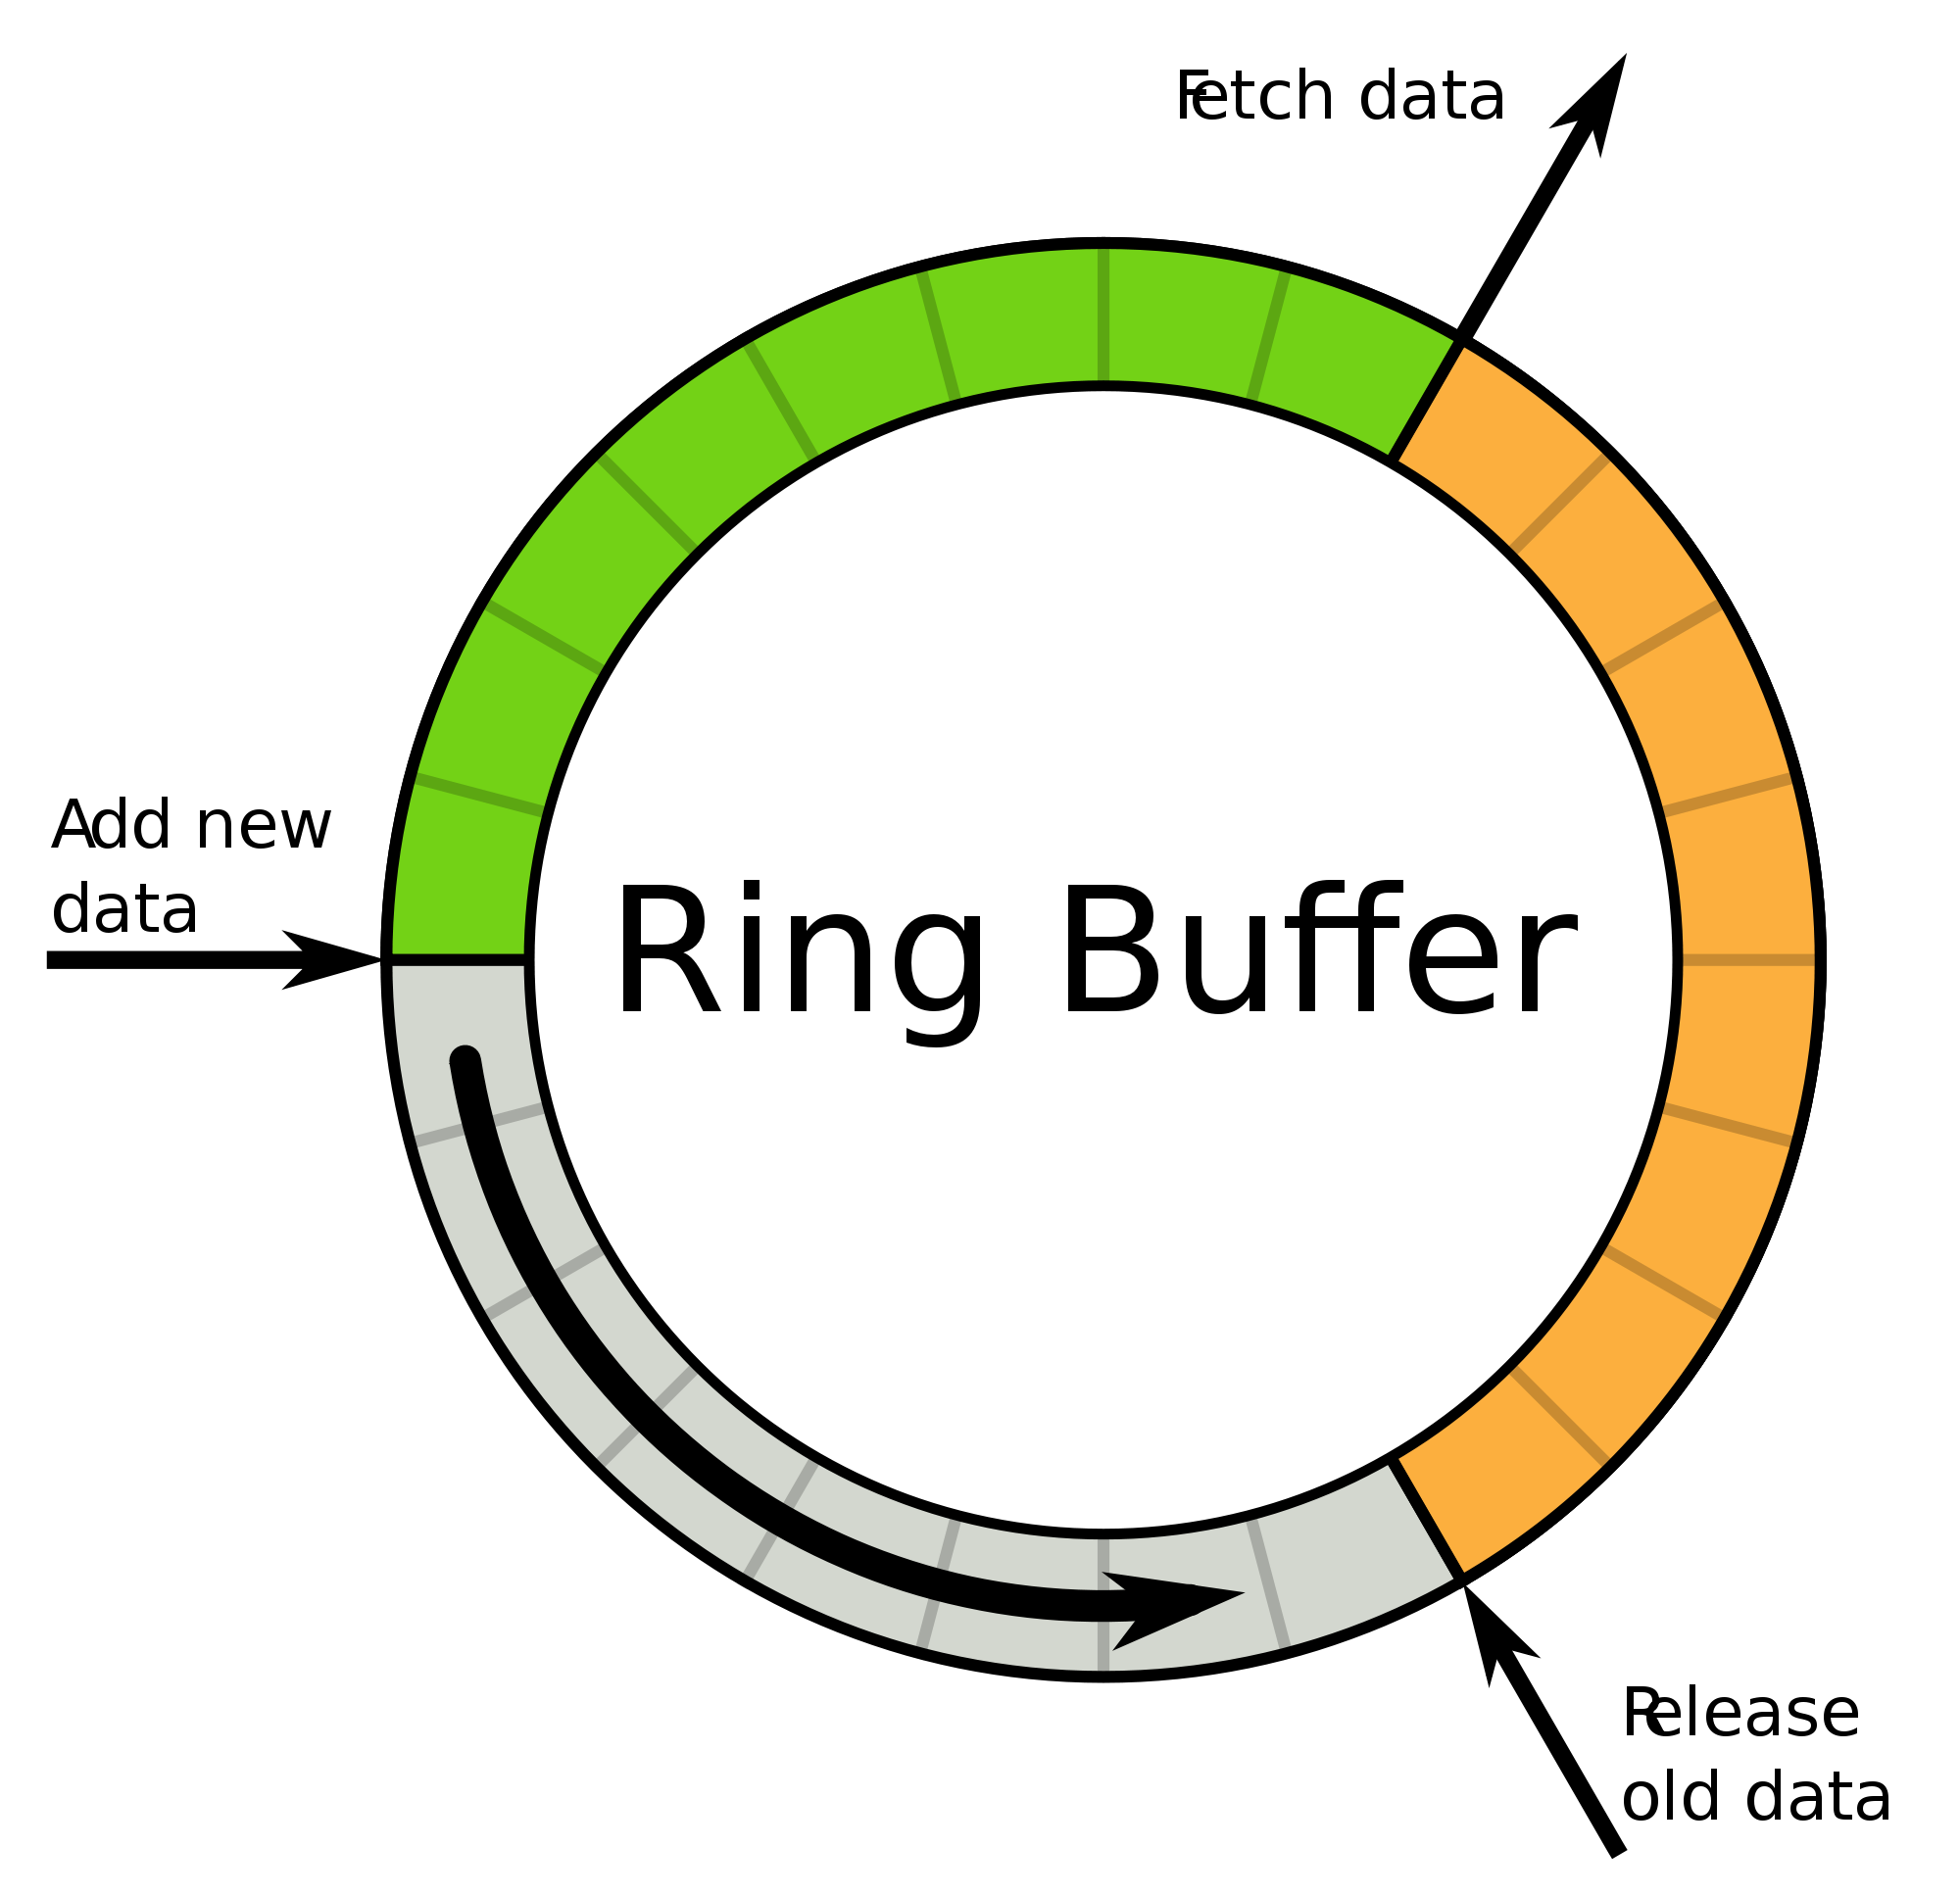
\includegraphics[width=\columnwidth]{Ringbuffer}
                \end{figure}
            \end{columns}
			\pause
		   \begin{figure}
				\begin{center}
				\begin{picture}(120,45)
					%boxes
					\setcounter{iXBlockSize}{11}
					\setcounter{iYBlockSize}{6}
					\setcounter{iYOffset}{40}
					\setcounter{iXOffset}{-4}
					\put(\value{iXOffset},\value{iYOffset}){\footnotesize{\shortstack[c]{i}}}
					\addtocounter{iXOffset}{\value{iXBlockSize}}
					\put(\value{iXOffset}, \value{iYOffset}){\framebox(\value{iXBlockSize},\value{iYBlockSize}){\tiny{$x_{i-1}$}}}
					\addtocounter{iXOffset}{\value{iXBlockSize}}
					\put(\value{iXOffset}, \value{iYOffset}){\framebox(\value{iXBlockSize},\value{iYBlockSize}){\tiny{$x_{i-2}$}}}
					\addtocounter{iXOffset}{\value{iXBlockSize}}
					\put(\value{iXOffset}, \value{iYOffset}){\framebox(\value{iXBlockSize},\value{iYBlockSize}){\tiny{$x_{i-3}$}}}
					\addtocounter{iXOffset}{\value{iXBlockSize}}
					\put(\value{iXOffset}, \value{iYOffset}){\framebox(\value{iXBlockSize},\value{iYBlockSize}){\tiny{$\ldots$}}}
					\addtocounter{iXOffset}{\value{iXBlockSize}}
					\put(\value{iXOffset}, \value{iYOffset}){\framebox(\value{iXBlockSize},\value{iYBlockSize}){\tiny{$x_{i-M+1}$}}}
					\addtocounter{iXOffset}{\value{iXBlockSize}}
					\put(\value{iXOffset}, \value{iYOffset}){\framebox(\value{iXBlockSize},\value{iYBlockSize}){\tiny{$x_{i-M}$}}}
					\addtocounter{iXOffset}{\value{iXBlockSize}}
					\put(\value{iXOffset}, \value{iYOffset}){\framebox(\value{iXBlockSize},\value{iYBlockSize}){\tiny{$x_{i-M-1}$}}}
					\addtocounter{iXOffset}{\value{iXBlockSize}}
					\put(\value{iXOffset}, \value{iYOffset}){\framebox(\value{iXBlockSize},\value{iYBlockSize}){\tiny{$\ldots$}}}
					\addtocounter{iXOffset}{\value{iXBlockSize}}
					\put(\value{iXOffset}, \value{iYOffset}){\framebox(\value{iXBlockSize},\value{iYBlockSize}){\tiny{$x_{i-L}$}}}
		  
					\put(67, 36){\vector(0,1){4}}
					\put(100, 36){\vector(0,1){4}}
					\put(68, 37){\footnotesize{\shortstack[c]{$n_\mathrm{r}$}}}
					\put(101, 37){\footnotesize{\shortstack[c]{$n_\mathrm{w}$}}}

					\pause
					\addtocounter{iYOffset}{-12}
					\setcounter{iXOffset}{-4}
					\put(\value{iXOffset},\value{iYOffset}){\footnotesize{\shortstack[c]{i+1}}}
					\addtocounter{iXOffset}{\value{iXBlockSize}}
					\put(\value{iXOffset}, \value{iYOffset}){\framebox(\value{iXBlockSize},\value{iYBlockSize}){\tiny{$x_{i-1}$}}}
					\addtocounter{iXOffset}{\value{iXBlockSize}}
					\put(\value{iXOffset}, \value{iYOffset}){\framebox(\value{iXBlockSize},\value{iYBlockSize}){\tiny{$x_{i-2}$}}}
					\addtocounter{iXOffset}{\value{iXBlockSize}}
					\put(\value{iXOffset}, \value{iYOffset}){\framebox(\value{iXBlockSize},\value{iYBlockSize}){\tiny{$x_{i-3}$}}}
					\addtocounter{iXOffset}{\value{iXBlockSize}}
					\put(\value{iXOffset}, \value{iYOffset}){\framebox(\value{iXBlockSize},\value{iYBlockSize}){\tiny{$\ldots$}}}
					\addtocounter{iXOffset}{\value{iXBlockSize}}
					\put(\value{iXOffset}, \value{iYOffset}){\framebox(\value{iXBlockSize},\value{iYBlockSize}){\tiny{$x_{i-M+1}$}}}
					\addtocounter{iXOffset}{\value{iXBlockSize}}
					\put(\value{iXOffset}, \value{iYOffset}){\framebox(\value{iXBlockSize},\value{iYBlockSize}){\tiny{$x_{i-M}$}}}
					\addtocounter{iXOffset}{\value{iXBlockSize}}
					\put(\value{iXOffset}, \value{iYOffset}){\framebox(\value{iXBlockSize},\value{iYBlockSize}){\tiny{$x_{i-M-1}$}}}
					\addtocounter{iXOffset}{\value{iXBlockSize}}
					\put(\value{iXOffset}, \value{iYOffset}){\framebox(\value{iXBlockSize},\value{iYBlockSize}){\tiny{$\ldots$}}}
					\addtocounter{iXOffset}{\value{iXBlockSize}}
					\put(\value{iXOffset}, \value{iYOffset}){\framebox(\value{iXBlockSize},\value{iYBlockSize}){\tiny{\color{gtgold}{$x_{i}$}}}}
		  
					\put(56, 24){\vector(0,1){4}}
					\put(89, 24){\vector(0,1){4}}
					\put(57, 25){\footnotesize{\shortstack[c]{$n_\mathrm{r}$}}}
					\put(90, 25){\footnotesize{\shortstack[c]{$n_\mathrm{w}$}}}
		 
					\pause
					\addtocounter{iYOffset}{-12}
					\setcounter{iXOffset}{-4}
					\put(\value{iXOffset},\value{iYOffset}){\footnotesize{\shortstack[c]{i+L-3}}}
					\addtocounter{iXOffset}{\value{iXBlockSize}}
					\put(\value{iXOffset}, \value{iYOffset}){\framebox(\value{iXBlockSize},\value{iYBlockSize}){\tiny{$x_{i-1}$}}}
					\addtocounter{iXOffset}{\value{iXBlockSize}}
					\put(\value{iXOffset}, \value{iYOffset}){\framebox(\value{iXBlockSize},\value{iYBlockSize}){\tiny{$x_{i-2}$}}}
					\addtocounter{iXOffset}{\value{iXBlockSize}}
					\put(\value{iXOffset}, \value{iYOffset}){\framebox(\value{iXBlockSize},\value{iYBlockSize}){\tiny{$x_{i-3}$}}}
					\addtocounter{iXOffset}{\value{iXBlockSize}}
					\put(\value{iXOffset}, \value{iYOffset}){\framebox(\value{iXBlockSize},\value{iYBlockSize}){\tiny{$\ldots$}}}
					\addtocounter{iXOffset}{\value{iXBlockSize}}
					\put(\value{iXOffset}, \value{iYOffset}){\framebox(\value{iXBlockSize},\value{iYBlockSize}){\tiny{$x_{i+L-M-1}$}}}
					\addtocounter{iXOffset}{\value{iXBlockSize}}
					\put(\value{iXOffset}, \value{iYOffset}){\framebox(\value{iXBlockSize},\value{iYBlockSize}){\tiny{$x_{i+L-M-2}$}}}
					\addtocounter{iXOffset}{\value{iXBlockSize}}
					\put(\value{iXOffset}, \value{iYOffset}){\framebox(\value{iXBlockSize},\value{iYBlockSize}){\tiny{$x_{i+L-M-3}$}}}
					\addtocounter{iXOffset}{\value{iXBlockSize}}
					\put(\value{iXOffset}, \value{iYOffset}){\framebox(\value{iXBlockSize},\value{iYBlockSize}){\tiny{$\ldots$}}}
					\addtocounter{iXOffset}{\value{iXBlockSize}}
					\put(\value{iXOffset}, \value{iYOffset}){\framebox(\value{iXBlockSize},\value{iYBlockSize}){\tiny{$x_{i}$}}}
			
					\put(78, 12){\vector(0,1){4}}
					\put(34, 12){\vector(0,1){4}}
					\put(79, 13){\footnotesize{\shortstack[c]{$n_\mathrm{r}$}}}
					\put(35, 13){\footnotesize{\shortstack[c]{$n_\mathrm{w}$}}}
				  
				\end{picture}
				\end{center}
			\end{figure}
		\end{frame}

		\begin{frame}{modulated effects}{introduction: modulated delay line}
			\begin{figure}
				\begin{center}
				\begin{picture}(30,10)

					%boxes
					\put(10,0){\framebox(10,10){\footnotesize{$z^{-M}$}}}

					%vectors diagonal
					\put(10,-4){\line(1,2){2}}
					\put(17,10){\vector(1,2){2}}
					
					%lines horizontal
					\put(0,5){\vector(1,0){10}}
					\put(20,5){\vector(1,0){10}}

					%text
					\put(0,8){\footnotesize{\shortstack[c]{x(i)}}}
					\put(30,8){\footnotesize{\shortstack[c]{y(i)}}}

				\end{picture}
				\end{center}
			\end{figure}
			\pause
			\begin{equation*}
				n.frac = M \color{gtgold}{+ A\cdot \sin\left( 2\pi \frac{f_{mod}}{f_s}i \right)}
			\end{equation*}
			
			\begin{itemize}
				\item	$M$: static delay in samples
				\item	$A$: modulation amplitude in samples
				\item	$f_{mod}$: modulation frequency in Hertz
				\item	$\sin$: oscillator function
			\end{itemize}
		\end{frame}

		\begin{frame}{modulated effects}{introduction: fractional delay line 1/4}
			
			\begin{itemize}
				\item	\textbf{problem}
					\begin{itemize}
						\item	(modulated) read index may be \textit{between} samples
						\item	rounding to integer index causes artifacts
							\begin{equation*}
								\hat{y}(i) = x(i - n.frac)
							\end{equation*}
					\end{itemize}
				\pause
				\item	\textbf{solution}
					\begin{itemize}
						\item	interpolate
							\begin{itemize}
								\item	linear interpolation
								\item	all pass interpolation
								\item	cubic, sinc, etc.\ interpolation
							\end{itemize}
					\end{itemize}
			\end{itemize}
		\end{frame}

		\begin{frame}{modulated effects}{introduction: fractional delay line 2/4}
			\begin{figure}
				\centerline{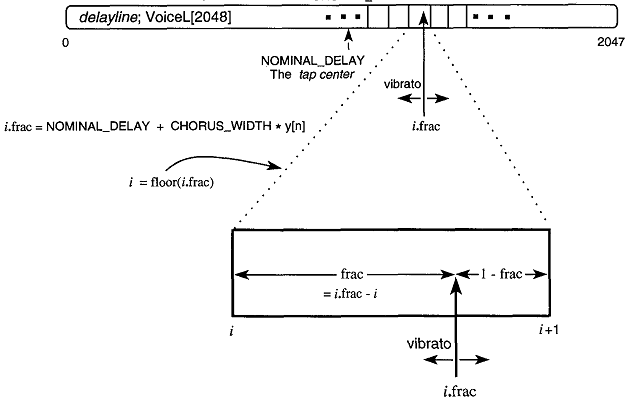
\includegraphics[scale=.6]{graph/frac_delay_line}}
				\label{fig:frac_delay_line}
			\end{figure}
		\end{frame}

		\begin{frame}{modulated effects}{introduction: fractional delay line 3/4}
			\textbf{linear interpolation}
			\begin{itemize}
				\item	simple to implement
				\item	works well if $f_{mod} << f_s$
			\pause
			\item	target delay: $i.frac$
				\begin{eqnarray*}
					\hat{y}(i) &=& x(i - n.frac)\\
					\pause
					n &=& floor(n.frac)\\
					frac &=& n.frac - n\\
					\pause
					\hat{y}(i) &=& x(i-n + 1)\cdot frac + x(i-n)\cdot (1-frac)
				\end{eqnarray*}
			\end{itemize}
		\end{frame}

		\begin{frame}{modulated effects}{linear interpolation: audio examples}
			\begin{itemize}
				\item   \textbf{original}: \includeaudio{sv}
				\smallskip
				\item   \textbf{6\% speed-up}: \includeaudio{sv@106}
				\smallskip
				\item   \textbf{6\% slow-down}: \includeaudio{sv@94}
			\end{itemize}
		\end{frame}

    \section{vibrato \& more}
		\begin{frame}{modulated effects}{vibrato}
			\begin{figure}
				\begin{center}
				\begin{picture}(30,10)

					%boxes
					\put(10,0){\framebox(10,10){\footnotesize{$z^{-M}$}}}

					%vectors diagonal
					\put(10,-4){\line(1,2){2}}
					\put(17,10){\vector(1,2){2}}
					
					%lines horizontal
					\put(0,5){\vector(1,0){10}}
					\put(20,5){\vector(1,0){10}}

					%text
					\put(0,8){\footnotesize{\shortstack[c]{x(i)}}}
					\put(30,8){\footnotesize{\shortstack[c]{y(i)}}}

				\end{picture}
				\end{center}
			\end{figure}
			\pause
			\flushright{\includeaudio{svVibrato}}
			
			\begin{itemize}
				\item	$M = any$
				\item	$A = \unit[200]{samples}$
				\item	$f_{mod} = \unit[1]{Hz}$
			\end{itemize}
		\end{frame}

		\begin{frame}{modulated effects}{vibrato + input signal}
			\begin{figure}
				\begin{center}
				\begin{picture}(30,20)

					%boxes
					\put(10,0){\framebox(10,10){\footnotesize{$z^{-M}$}}}

					%vectors diagonal
					\put(10,-4){\line(1,2){2}}
					\put(17,10){\vector(1,2){2}}
					
					%lines horizontal
					\put(0,5){\vector(1,0){10}}
					\put(20,5){\vector(1,0){4}}
					\put(26,5){\vector(1,0){3}}
					\put(31,5){\vector(1,0){4}}
					\put(5,15){\vector(1,0){9}}
					\put(16,15){\line(1,0){14}}
					
					%lines vertical
					\put(5,5){\line(0,1){10}}
					\put(30,15){\vector(0,-1){9}}
					
					%circles
					\put(13.5,14){$\otimes$} %15,15
					\put(23.5,4){$\otimes$} % 25,5
					\put(28.5,4){$\oplus$} % 30,5
					
					\put(5,5){\circle*{1}}

					%text
					\put(-2,8){\footnotesize{\shortstack[c]{x(i)}}}
					\put(35,8){\footnotesize{\shortstack[c]{y(i)}}}
					\put(16,16){\footnotesize{\shortstack[c]{BL}}}
					\put(25,7){\footnotesize{\shortstack[c]{FF}}}

				\end{picture}
				\end{center}
			\end{figure}
			\only<1>{
				\begin{itemize}
					\item[]
					\item[]
					\item[]
					\item[]
					\item[]
					\item[]
				\end{itemize}
			}
			\only<2>{
				\textbf{slapback}
				
				\vspace{-8mm}
				\flushright{\includeaudio{svSlapback}}
				\begin{itemize}
					\item	$f_{mod} = 0$
					\item	$ A = 0$
					\item	$ M = \unit[20]{ms}$
					\item	$BL = 0.7$
					\item	$FF = 0.7$
				\end{itemize}
			}
			\only<3>{
				\textbf{simple echo}
				
				\vspace{-8mm}
				\flushright{\includeaudio{svEcho}}
				\begin{itemize}
					\item	$f_{mod} = 0$
					\item	$ A = 0$
					\item	$ M = \unit[50]{ms}$
					\item	$BL = 0.7$
					\item	$FF = 0.7$
				\end{itemize}
			}
			\only<4>{
				\textbf{simple flanger}
				
				\vspace{-8mm}
				\flushright{\includeaudio{svFlanger}}
				\begin{itemize}
					\item	$f_{mod} = \unit[0.2]{Hz}$
					\item	$ A = \unit[2]{ms}$
					\item	$ M = 0$
					\item	$BL = 0.7$
					\item	$FF = 0.7$
				\end{itemize}
			}
			\only<5>{
				\textbf{simple chorus}
				
				\vspace{-8mm}
				\flushright{\includeaudio{svChorus}}
				\begin{itemize}
					\item	$f_{mod} = \unit[1.5]{Hz}$
					\item	$ A = \unit[2]{ms}$
					\item	$ M = \unit[2]{ms}$
					\item	$BL = 1.0$
					\item	$FF = 0.7$
				\end{itemize}
			}
		\end{frame}

		\begin{frame}{modulated effects}{modulated effect with feedback path}
			\begin{figure}[!hbt]
				\begin{center}
				\begin{picture}(30,40)

					%boxes
					\put(10,20){\framebox(10,10){\footnotesize{$z^{-M}$}}}
					\put(3,6){\framebox(8,8){\footnotesize{$H(z)$}}}

					%vectors diagonal
					\put(10,16){\line(1,2){2}}
					\put(17,30){\vector(1,2){2}}
					
					%lines horizontal
					\put(0,25){\vector(1,0){10}}
					\put(20,25){\vector(1,0){4}}
					\put(26,25){\vector(1,0){3}}
					\put(31,25){\vector(1,0){4}}
					\put(5,35){\vector(1,0){9}}
					\put(16,35){\line(1,0){14}}
					
					\put(0,10){\line(1,0){3}}
					\put(15,10){\vector(-1,0){4}}
					\put(-5,25){\vector(1,0){4}}
					
					%lines vertical
					\put(5,25){\line(0,1){10}}
					\put(30,35){\vector(0,-1){9}}
					
					\put(0,10){\vector(0,1){6}}
					\put(0,18){\vector(0,1){6}}
					\put(15,20){\line(0,-1){10}}
					
					%circles
					\put(13.5,34){$\otimes$} %15,15
					\put(23.5,24){$\otimes$} % 25,5
					\put(28.5,24){$\oplus$} % 30,25
					\put(-1.5,16){$\otimes$} % 0,17
					\put(-1.5,24){$\oplus$} % 0,25
					
					\put(5,25){\circle*{1}}

					%text
					\put(-6,28){\footnotesize{\shortstack[c]{x(i)}}}
					\put(35,28){\footnotesize{\shortstack[c]{y(i)}}}
					\put(16,36){\footnotesize{\shortstack[c]{BL}}}
					\put(25,27){\footnotesize{\shortstack[c]{FF}}}
					\put(1,18){\footnotesize{\shortstack[c]{FB}}}

				\end{picture}
				\end{center}
			\end{figure}
			\vspace{-10mm}
			\only<1>{
				\begin{itemize}
					\item[]
					\item[]
					\item[]
					\item[]
					\item[]
					\item[]
				\end{itemize}
			}
			\only<2>{
				\textbf{simple flanger with feedback}
				
				\vspace{-8mm}
				\flushright{\includeaudio{svFlangerFb}}
				\begin{itemize}
					\item	$f_{mod} = \unit[0.1]{Hz}$
					\item	$ A = \unit[5]{ms}$
					\item	$ M = 0$
					\item	$BL = 0.7$
					\item	$FF = 0.7$
					\item	$FB = -0.7$
				\end{itemize}
			}
			\only<3>{
				\textbf{white chorus}
				
				\vspace{-8mm}
				\flushright{\includeaudio{svWhiteChorus}}
				\begin{itemize}
					\item	$f_{mod} = \unit[1.5]{Hz}$
					\item	$ A = \unit[2]{ms}$
					\item	$ M = \unit[2]{ms}$
					\item	$BL = 0.7$
					\item	$FF = 1.0$
					\item	$FB = -0.7$
				\end{itemize}
			}
		\end{frame}

		\begin{frame}{modulated effects}{chorus: implementation variant}
						\begin{figure}[!hbt]
							\begin{center}
							\begin{picture}(50,80)
				
								%boxes
								\put(25,50){\framebox(7,6){\footnotesize{$z^{-M_1}$}}}
								\put(25,38){\framebox(7,6){\footnotesize{$z^{-M_2}$}}}
								\put(28,28){\shortstack[c]{$\vdots$}}
								\put(25,14){\framebox(7,6){\footnotesize{$z^{-M_N}$}}}
					
								%vectors diagonal
								%25,50
								\put(25,46){\line(1,2){2}}
								\put(30,56){\vector(1,2){2}}
								%25,38
								\put(25,34){\line(1,2){2}}
								\put(30,44){\vector(1,2){2}}
								%25,14
								\put(25,10){\line(1,2){2}}
								\put(30,20){\vector(1,2){2}}
				
								%lines horizontal
								\put(5,65){\vector(1,0){22.5}}
								\put(29.5,65){\vector(1,0){11.5}}
								\put(43,65){\vector(1,0){10}}
								
								\put(15,53){\vector(1,0){10}}
								\put(32,53){\vector(1,0){3.5}}
								\put(38,53){\vector(1,0){3}}
								
								\put(15,41){\vector(1,0){10}}
								\put(32,41){\vector(1,0){3.5}}
								\put(38,41){\vector(1,0){3}}
								
								\put(15,29){\vector(1,0){10}}
								\put(32,29){\vector(1,0){3.5}}
								\put(38,29){\vector(1,0){3}}
								
								\put(15,17){\vector(1,0){10}}
								\put(32,17){\line(1,0){10}}
				
								%lines vertical
								\put(15,65){\line(0,-1){48}}
								
								\put(42,54){\vector(0,1){10}}
								%\put(42,60){\vector(0,1){4}}
								
								\put(42,42){\vector(0,1){10}}
								%\put(42,48){\vector(0,1){4}}
								
								\put(42,30){\vector(0,1){10}}
								%\put(42,36){\vector(0,1){4}}
								
								\put(42,17){\vector(0,1){5}}
								\put(42,24){\vector(0,1){4}}
								
								%circles
								\put(27,64){$\otimes$}
								\put(40.5,64){$\oplus$} % 42-20
								\put(40.5,52){$\oplus$} % 42-20
								\put(40.5,40){$\oplus$} % 42-20
								\put(40.5,28){$\oplus$} % 42-20
								
								\put(35,52){$\otimes$}
								\put(35,40){$\otimes$}
								\put(35,28){$\otimes$}
								\put(40.5,22){$\otimes$}
								
								\put(15,65){\circle*{1}}
								\put(15,53){\circle*{1}}
								\put(15,41){\circle*{1}}
								\put(15,29){\circle*{1}}
				
								%text
								\put(26,68){\footnotesize{\shortstack[c]{$BL$}}}
								\put(36,56){\footnotesize{\shortstack[c]{$FF_1$}}}
								\put(36,44){\footnotesize{\shortstack[c]{$FF_2$}}}
								\put(36,32){\footnotesize{\shortstack[c]{$FF$}}}
								\put(44,21){\footnotesize{\shortstack[c]{$FF_N$}}}
				
								\put(4,67){\footnotesize{\shortstack[c]{x(i)}}}
								\put(52,67){\footnotesize{\shortstack[c]{y(i)}}}
				
							\end{picture}
							\end{center}
						\end{figure}
		\end{frame}

		\begin{frame}{modulated effects}{modulated effects: typical variants}
			\begin{figure}
				\begin{center}
				\begin{picture}(30,40)

					%boxes
					\put(10,20){\framebox(10,10){\footnotesize{$z^{-M}$}}}
					\put(3,6){\framebox(8,8){\footnotesize{$H(z)$}}}

					%vectors diagonal
					\put(10,16){\line(1,2){2}}
					\put(17,30){\vector(1,2){2}}
					
					%lines horizontal
					\put(0,25){\vector(1,0){10}}
					\put(20,25){\vector(1,0){4}}
					\put(26,25){\vector(1,0){3}}
					\put(31,25){\vector(1,0){4}}
					\put(5,35){\vector(1,0){9}}
					\put(16,35){\line(1,0){14}}
					
					\put(0,10){\line(1,0){3}}
					\put(15,10){\vector(-1,0){4}}
					\put(-5,25){\vector(1,0){4}}
					
					%lines vertical
					\put(5,25){\line(0,1){10}}
					\put(30,35){\vector(0,-1){9}}
					
					\put(0,10){\vector(0,1){6}}
					\put(0,18){\vector(0,1){6}}
					\put(15,20){\line(0,-1){10}}
					
					%circles
					\put(13.5,34){$\otimes$} %15,15
					\put(23.5,24){$\otimes$} % 25,5
					\put(28.5,24){$\oplus$} % 30,25
					\put(-1.5,16){$\otimes$} % 0,17
					\put(-1.5,24){$\oplus$} % 0,25
					
					\put(5,25){\circle*{1}}

					%text
					\put(-6,28){\footnotesize{\shortstack[c]{x(i)}}}
					\put(35,28){\footnotesize{\shortstack[c]{y(i)}}}
					\put(16,36){\footnotesize{\shortstack[c]{BL}}}
					\put(25,27){\footnotesize{\shortstack[c]{FF}}}
					\put(1,18){\footnotesize{\shortstack[c]{FB}}}

				\end{picture}
				\end{center}
			\end{figure}
			\begin{itemize}
				\item	add low pass/transfer function to feedback path
				\item	use stereo feedback
			\end{itemize}
		\end{frame}

    \section{modulation}
		\begin{frame}{modulated effects}{modulated effects: modulation signal}
			\begin{itemize}
				\item	\textbf{shape}
					\begin{itemize}
						\item	low frequency 
						\item	\textit{sinusoidal} (typically) or \textit{noise} (low pass filtered)
						
					\end{itemize}
				\pause
				\bigskip
				\item	\textbf{phase}
					\begin{itemize}
						\item	\textbf{phase response} becomes perceptually relevant when
							\begin{itemize}
								\item   2 or more signals are added
								\item   phase is time-variant
								\item   phase shift between channels (localization)
							\end{itemize}
					\end{itemize}
			\end{itemize}
		\end{frame}

    \section{phaser \& wah-wah}
		\begin{frame}{modulated effects}{modulated effects: phaser}
			\begin{itemize}
				\item	sounds similar to delay line effects
				\item	but: different implementation
				\pause
					\begin{itemize}
						\item	notch filters
					\begin{figure}
						\begin{center}
						\begin{picture}(50,20)
			
							%boxes
							\put(16,5){\framebox(7,6){\footnotesize{NO}}}
							\put(25,5){\framebox(7,6){\footnotesize{NO}}}
							\put(34,5){\framebox(7,6){\footnotesize{NO}}}
			
							%vectors diagonal
							\put(16,2){\line(1,2){1.8}}
							\put(21,11){\vector(1,2){2}}
							\put(25,2){\line(1,2){1.8}}
							\put(30,11){\vector(1,2){2}}
							\put(34,2){\line(1,2){1.8}}
							\put(39,11){\vector(1,2){2}}
			
							%lines horizontal
							\put(5,20){\vector(1,0){22.5}}
							\put(29.5,20){\vector(1,0){11.5}}
							\put(43,20){\vector(1,0){10}}
							
							\put(15,8){\vector(1,0){1}}
							\put(23,8){\vector(1,0){2}}
							\put(32,8){\vector(1,0){2}}
							\put(41,8){\line(1,0){1}}
			
							%lines vertical
							\put(15,20){\line(0,-1){12}}
							\put(42,8){\vector(0,1){4}}
							\put(42,14){\vector(0,1){5}}
							
							%circles
							\put(27,19){$\otimes$}
							\put(40.5,19){$\oplus$} % 42-20
							\put(40.5,12){$\otimes$}
							
							\put(15,20){\circle*{1}}
			
							%text
							\put(29,21){\footnotesize{\shortstack[c]{$d$}}}
							\put(43,14){\footnotesize{\shortstack[c]{$e$}}}
			
							\put(4,22){\footnotesize{\shortstack[c]{x(i)}}}
							\put(52,22){\footnotesize{\shortstack[c]{y(i)}}}
			
						\end{picture}
						\end{center}
					\end{figure}
						\pause
						\item	all pass filters

					\begin{figure}
						\begin{center}
						\begin{picture}(50,20)
			
							%boxes
							\put(16,5){\framebox(7,6){\footnotesize{AP}}}
							\put(25,5){\framebox(7,6){\footnotesize{AP}}}
							\put(34,5){\framebox(7,6){\footnotesize{AP}}}
			
							%vectors diagonal
							\put(16,2){\line(1,2){1.8}}
							\put(21,11){\vector(1,2){2}}
							\put(25,2){\line(1,2){1.8}}
							\put(30,11){\vector(1,2){2}}
							\put(34,2){\line(1,2){1.8}}
							\put(39,11){\vector(1,2){2}}
			
							%lines horizontal
							\put(5,20){\vector(1,0){38}}
							\put(45,20){\vector(1,0){4}}
							\put(51,20){\vector(1,0){9}}
							
							\put(10,8){\vector(1,0){6}}
							\put(23,8){\vector(1,0){2}}
							\put(32,8){\vector(1,0){2}}
							\put(41,8){\vector(1,0){2}}
							\put(45,8){\line(1,0){5}}

							\put(50,0){\vector(-1,0){5}}
							\put(43,0){\line(-1,0){33}}
			
							%lines vertical
							\put(10,20){\vector(0,-1){11}}
							\put(50,0){\vector(0,1){19}}
							\put(10,0){\vector(0,1){7}}
							
							%circles
							\put(42.5,19){$\otimes$}
							\put(48.5,19){$\oplus$} % 50,20
							\put(8.5,7){$\oplus$} 
							\put(42.5,7){$\otimes$}
							\put(42.5,-1){$\otimes$}
							
							\put(10,20){\circle*{1}}
							\put(50,8){\circle*{1}}
			
							%text
							\put(45,21){\footnotesize{\shortstack[c]{$d$}}}
							\put(45,9){\footnotesize{\shortstack[c]{$e$}}}
							\put(45,1){\footnotesize{\shortstack[c]{$fb$}}}
			
							\put(4,22){\footnotesize{\shortstack[c]{x(i)}}}
							\put(52,22){\footnotesize{\shortstack[c]{y(i)}}}
			
						\end{picture}
						\end{center}
					\end{figure}
						\pause
						\item[]	%audio example (all pass)\\
			$f_{mod} = \unit[1]{Hz}, N = 5, M = {2}{ms}, d = 0.5, e = 0.5, fb = 0.5$
			\includeaudio{svPhaser}
			\end{itemize}
			\end{itemize}
		\end{frame}

		\begin{frame}{modulated effects}{modulated effects: wah-wah}
					\begin{figure}[!hbt]
						\begin{center}
						\begin{picture}(50,30)
			
							%boxes
							\put(25,5){\framebox(7,6){\footnotesize{$BP$}}}
							
							%diagonal
							\put(25,2){\line(1,2){1.8}}
							\put(30,11){\vector(1,2){2}}
			
							%lines horizontal
							\put(5,20){\vector(1,0){22.5}}
							\put(29.5,20){\vector(1,0){11.5}}
							\put(43,20){\vector(1,0){10}}
							
							\put(15,8){\vector(1,0){10}}
							\put(32,8){\line(1,0){10}}
			
							%lines vertical
							\put(15,20){\line(0,-1){12}}
							\put(42,8){\vector(0,1){4}}
							\put(42,14){\vector(0,1){5}}
							
							%circles
							\put(27,19){$\otimes$}
							\put(40.5,19){$\oplus$} % 42-20
							\put(40.5,12){$\otimes$}
							
							\put(15,20){\circle*{1}}
			
							%text
							\put(29,21){\footnotesize{\shortstack[c]{1-g}}}
							\put(44,13){\footnotesize{\shortstack[c]{g}}}
			
							\put(4,22){\footnotesize{\shortstack[c]{x(i)}}}
							\put(52,22){\footnotesize{\shortstack[c]{y(i)}}}
			
						\end{picture}
						\end{center}
					\end{figure}
					\begin{itemize}
						\item   'modulated' by pedal
						\item   often a biquad implementation
						\item   not really a bandpass 
							\begin{itemize}
								\item changes shape depending on frequency (resonant at low freqs, broad at high freqs)
							\end{itemize}
					\end{itemize}
		\end{frame}



        \section{summary}
        \begin{frame}{modulated effects}{summary}
            \begin{itemize}
                \item	most modulated effects are based on \textbf{delay lines}: 
                    \begin{itemize}
                        \item   input signal is added to a delayed version of itself
                        \item   delay time is modulated
                    \end{itemize}
                    
                \bigskip
                \item<2->	modulation is at very low frequencies (or manually controlled)
                    \begin{itemize}
                        \item   often sinusoidal
                    \end{itemize}
                \bigskip
                \item<3->	filters can also be used to create wanted phasing artifacts
                    \begin{itemize}
                        \item   all-pass and notch filters for phaser
                        \item   band-pass for wah-wah
                    \end{itemize}
            \end{itemize}
        \end{frame}


\end{document}

